\section{Deep Learning}
\subsection{Supervised Learning with Gradient Descent}
Machine learning is about solving problems we do not know how to solve directly.
Rather, we perform some kind of statistical inference.
In supervised machine learning, we are trying to learn a mapping from inputs to outputs, for example between the pixels of an image and the classification of that image.
Neural networks are a type of mapping known as a \textit{parametric} model.
I will outline here the general procedure for training such a model before detailing the specifics of neural networks themselves.

To first step to learning this mapping is to obtain some \(\{x_i \in \R^n, \ y_i \in \R^m\}_{i=1}^N\) data points to learn from, called the training data.
Then, we pick some functional representation, for example \(y = xw + b\), where \(w \in \R^{m \times n}, b \in \R^m\); meaning we approximate the true mapping as a linear function.
We will attempt to learn from the data the parameters \(w, b\) that best model the training data.
Note, \(\theta\) is often used as a single variable to denote all the parameters.
We will call our linear function given those parameters \(f_\theta : R^n \rightarrow R^m\).
It is often referred to as the hypothesis, model, or the network in the case of neural networks. The space of all possible \(\theta\) is known as the hypothesis space, weight space, or parameter space.

To conduct learning, we need a performance metric for our function and a method to optimise the parameters with respect to that metric. The performance metric is often referred to as a loss function, cost function, or error function; and evaluates how `good' the parameters are using the training data. We denote this loss function, \(L_\mathrm{D} : \Theta \rightarrow \R^+\), where \(\Theta\) is the set of all possible parameters and \(\mathrm{D}\) is the training data. Typically, the loss averages over data points as follows:

\begin{equation*}
    L_\mathrm{D}(\theta) = \frac{1}{N}\sum_{i=1}^N l(f_\theta(x_i),\, y_i)
\end{equation*}

where \(l : \R^m\times\R^m \rightarrow \R^+\) measures the `loss' between the training data outputs, known as the targets, and what \(f_{\theta}\) produced, for that specific data point. This could be the square-error loss \(l(o,\, t) = (o\,-\,t)^2\), for example.

Thus, the original problem has been reduced into an optimisation problem. Specifically, the objective is to minimise \(L_D\) with respect to \(\theta\).

We can do this using gradient descent \cite{Cauchy1847}. This is an iterative method that follows the line of steepest descent (the gradient) down the slope in small increments, often likened to placing a ball on the loss surface and watching it roll down to the minimum point. Formally, the procedure is to initialise our parameters to some \(\theta_0\) before iteratively applying the following update rule until we are satisfied with our parameters:

\begin{equation*}
    \theta_{k+1} = \theta_k + \eta((\nabla L_\mathrm{D})(\theta_k))^\top
\end{equation*}

Where \(\nabla L_\mathrm{D}\) is the Jacobian matrix of the loss with respect to the parameters, and \(\eta \in \R\) is a small, positive number known as the learning rate. Given sufficiently small \(\eta\), the sequence \(L_\mathrm{D}(\theta_0) \,\geq\, L_\mathrm{D}(\theta_1), \,\geq\, L_\mathrm{D}(\theta_2), \,\geq\, \ldots\) must converge to a local minimum of \(L_\mathrm{D}\).

\subsection{Mini-Batch Stochastic Gradient Descent}
Attempting to use gradient descent exactly as described above leads to some issues in the real-world. Firstly, every single weight update step requires iterating over the entire dataset to evaluate the loss. Real world datasets are very large, for example the ImageNet Large Scale Visual Recognition Challenge (ILSVRC) Object Localisation dataset has over 1.2 million images \cite{ILSVRC15}. Iterating over this entire dataset for a single weight update would be prohibitively slow. Secondly, recall gradient descent is only guaranteed to converge to the \textit{local} minima. For our simple example, the loss function is convex, so this is not a problem. However, to model complex real world problems, we need more expressive functional representations that can model highly complex non-linearities, leading to a non-convex loss. As an example, the loss surface of the VGG-56 \footnote{VGGNets are a popular neural network architecture for computer vision tasks. A VGGNet won the object localisation task of the ILSVRC in 2014.} network \cite{Simonyan2014} is visualised in Figure \ref{fig:2-vgg-loss}. Note it has many narrow local minima for gradient descent to get stuck in.

\begin{figure}[htb]
    \centering
    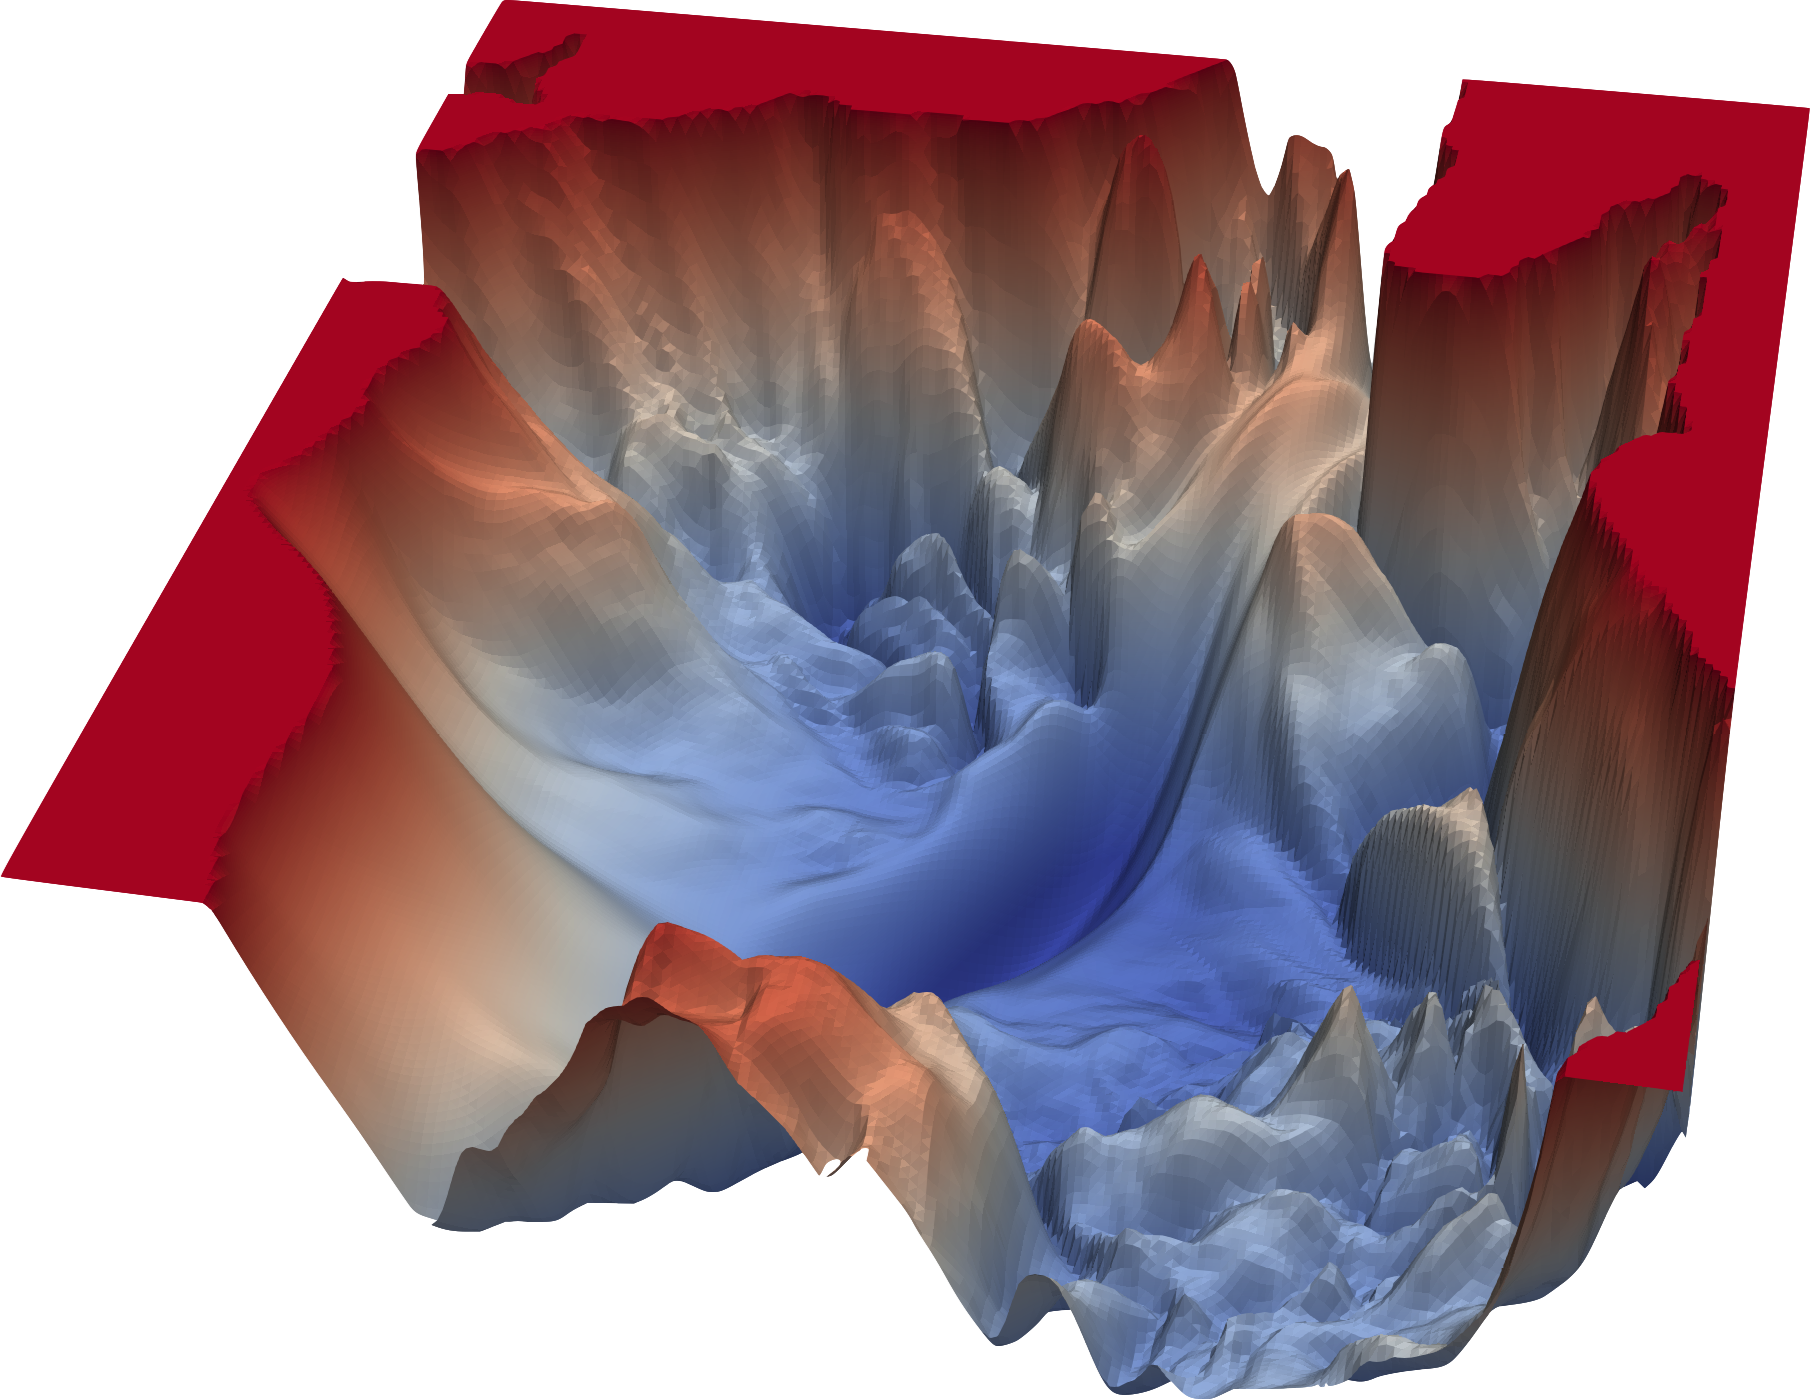
\includegraphics[width=0.7\linewidth]{vgg_56_loss.png}
    \caption{Visualisation of the loss function of VGG-56 \cite{Li2018}.}
    \label{fig:2-vgg-loss}
\end{figure}

To work around these problems, stochastic gradient descent (SGD) is used \cite{Bottou2018}. Rather than updating the parameters by computing the loss over the entire dataset, only a small `mini-batch' is used for one update step. This approximates true gradient descent and takes more steps to converge, but each step is now computationally tractable. Moreover, it means that on every update we are actually descending a different loss curve, \(L_\mathrm{B}\), defined by the mini-batch \(\mathrm{B}\subseteq \mathrm{D}\) we are working on, as opposed to always using the same loss curve \(L_\mathrm{D}\) that sums over all of the data. To see why this is beneficial, consider when after an update we have reached the local minima for that loss, but not the true global minima. On the next update, we are descending a different loss curve that likely does not have that exact local minima too, so we can ‘fall through it’ and continue towards the global minima.

\subsection*{A Note on Stochastic Gradient Descent in Practice}
I have outlined the SGD process used to train models in machine learning, which will be applied to neural networks in the next section and made memory-efficient in the remainder of this thesis.

It should be noted, however, that even SGD is not actually good enough by itself.
Much research goes into improving the optimisation methods of machine learning.
Commonly used techniques include dropout \cite{Srivastava2014}, L1/L2 regularisation \cite{Anders1992-weight-decay, Ng2004}, momentum \cite{Sutskever2013}, and Adam Optimisation \cite{Kingma2015-adam}.

None of these methods significantly affect the nature of the memory optimisations presented later, so I will not cover them here.

\subsection{Artificial Neural Networks}
The problems being solved today, such as computer vision tasks, are extremely difficult.
A simple linear function will not be able to sufficiently express the intricacies of the real underlying mapping being approximated.
We need a model that (i) can express complex non-linearities, (ii) has a continuous hypothesis space, and (iii) the hypothesis space is differentiable with respect to its parameters.
Neural networks satisfy these conditions and have been found to work very well.
They are the composition of many elementary non-linear operators, called \textit{neurons}.
An example of such a network is given in Figure \ref{fig:2-example-net}, repeated from the introduction.
\begin{figure}[h]
    \centering
    \hspace{0.5cm}
    \begin{subfigure}[]{0.4\textwidth}
        \centering
        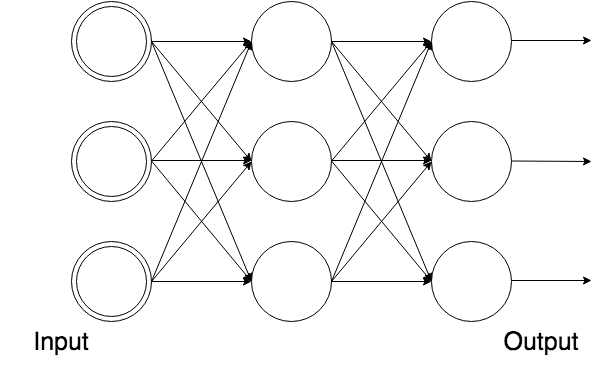
\includegraphics[width=\linewidth]{example_nn_neurons.png}
        \caption{At the individual neuron level.}
    \end{subfigure}%
    \hfill
    \begin{subfigure}[]{0.4\textwidth}
        \centering
        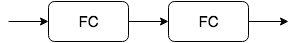
\includegraphics[width=\linewidth]{example_nn_layers.png}
        \caption{At the layer-wise level (\texttt{FC} means `fully connected').}
    \end{subfigure}%
    \hspace{0.5cm}
    \caption{Example ANN. The double circles denote variables rather than functions.}
    \label{fig:2-example-net}
\end{figure}
This network would be described as a feedforward/sequential/linear network of two fully-connected/dense layers.
This is because there are two layers of neurons in sequence, with each layer feeding the outputs of the previous layer to all of its neurons.

The function performed by an individual neuron is normally of the form:
\begin{equation*}
y = \sigma(w^\top x + b)
\end{equation*}
where \(\sigma : \R \rightarrow \R\) is called the \textit{activation function} or a \textit{threshold} and applies a non-linearity to the affine transform inside.
Examples include the Rectified Linear Unit (ReLU), \(\sigma(y) \,=\, \mathrm{max}(0,\, y)\);
and the sigmoid/logistic function, \(\sigma(y)\, =\, 1 / (1+e^{-y})\).

This is all it takes to describe a neural network, but they are incredibly powerful -
the Universal Approximation Theorom \cite{Cybenkot1989, Hornik1989}\cite[p.~105]{Mitchell1997-ML} states that any bounded continuous function can be approximated with arbitrarily small error (under a finite norm) by a network of just \textit{two} layers
\footnote{This does not say anything about the \textit{learnability} of the parameters of such networks though.}.

\subsection{Backpropagation}
How, then, do we train such a network?
To recap, we must minimise the loss with respect to the parameters of the model using gradient descent, which requires finding the partial derivates of the loss with respect to each parameter.
This was a trivial matter for a simple linear function, but, for a neural network, we need to get the partial derivates for the parameters \textit{at each neuron}.
This is easy too; as the neurons are just functions composed together, we can use the chain rule to find the derivatives for the parameters at each neuron.

Consider the example network in Figure \ref{fig:2-nn-chain-rule-forward}.
Then, we use the recursive formulas to obtain the desired derivates:

\begin{align*}
    \frac{\partial L}{\partial \theta_4} \,&=\, \frac{\partial L}{\partial f_4}\frac{\partial f_4}{\partial \theta_4} \,&&=\, \delta_4\frac{\partial f_4}{\partial \theta_4} \\[0.5em]
    \frac{\partial L}{\partial \theta_3} \,&=\, \frac{\partial L}{\partial f_4}\frac{\partial f_4}{\partial f_3}\frac{\partial f_3}{\partial \theta_3} \,&&=\, \delta_4\frac{\partial f_4}{\partial f_3}\frac{\partial f_3}{\partial \theta_3} \,&&&=\, \delta_3\frac{\partial f_3}{\partial \theta_3} \\[0.5em]
    \frac{\partial L}{\partial \theta_2} \,&=\, \frac{\partial L}{\partial f_4}\frac{\partial f_4}{\partial f_3}\frac{\partial f_3}{\partial f_2}\frac{\partial f_2}{\partial \theta_2} \,&&=\, \delta_3\frac{\partial f_3}{\partial f_2}\frac{\partial f_2}{\partial \theta_2} \,&&&=\, \delta_2\frac{\partial f_2}{\partial \theta_2} \\[0.5em]
    \frac{\partial L}{\partial \theta_1} \,&=\, \frac{\partial L}{\partial f_4}\frac{\partial f_4}{\partial f_3}\frac{\partial f_3}{\partial f_1}\frac{\partial f_1}{\partial \theta_1} \,&&=\, \delta_3\frac{\partial f_3}{\partial f_1}\frac{\partial f_1}{\partial \theta_1} \,&&&=\, \delta_1\frac{\partial f_1}{\partial \theta_1} \\[0.5em]
    \text{where}\\[0.6em]
    \delta_l &= \frac{\partial L}{\partial f_l}
\end{align*}

\begin{figure}[t]
    \centering
    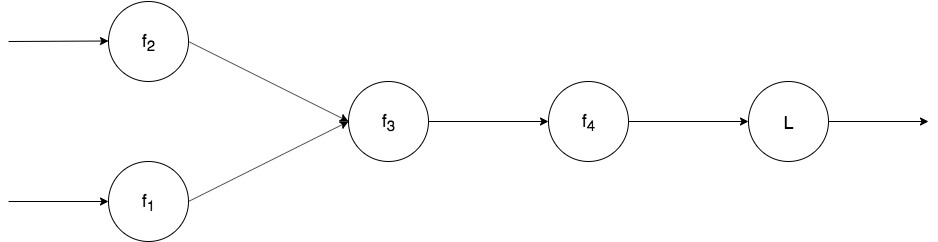
\includegraphics[width=0.9\linewidth]{chain_rule_forward_graph_only.jpg}
    \caption{An example network.}
    \label{fig:2-nn-chain-rule-forward}
\end{figure}

That is, we start at the end of the network and go backwards:
we use \(\delta_{l+1}\) to work out \(\delta_l\) and \(\frac{\partial L}{\partial \theta_l}\);
then use \(\delta_l\) to work out \(\delta_{l-1}\) and \(\frac{\partial L}{\partial \theta_{l-1}}\); and so on.
Thus, the \textit{deltas} are being propagated backwards, and so the process is known as \textit{backpropagation}.
Figure \ref{fig:2-nn-chain-rule-backward} shows the computational graph for this.
The `forward graph' is shown with the corresponding `backward graph' for computing the derivates using the chain rule.

\begin{figure}[htb]
    \centering
    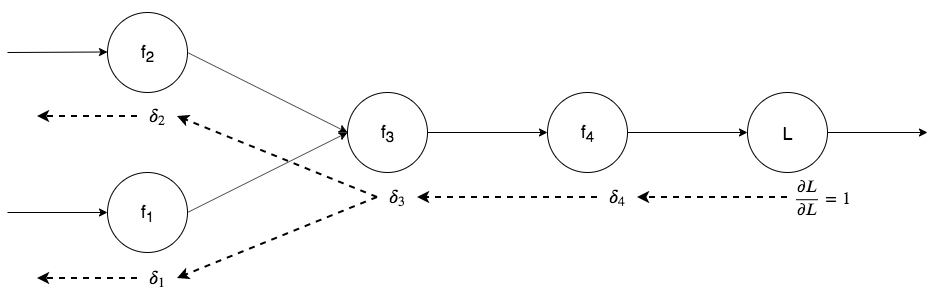
\includegraphics[width=0.9\linewidth]{chain_rule_backward_graph.png}
    \caption{Backpropagation on a simple network.}
    \label{fig:2-nn-chain-rule-backward}
\end{figure}


\subsection{The Computational Graph for Training a Network}
% let us fully derive comp graph. Specifically, we will use feedforward network of sigmoid-ed fully connected layers with a MSE loss. Note final layer directly feeding loss is unthresholded.
% Give definitions
% Give specific loss eqn
% Give update rules for one step of SGD
% Give full comp graph

Figure \ref{fig:2-nn-chain-rule-backward} merely shows how to backpropagate deltas.
It does not fully describe one step of training a neural network, for example it does not show the weight updates.

To derive the full graph, we must fully specify the update rules for backpropagation and gradient descent.


Consider an \(N\) layer network with any number of neurons per layer.
Let \(\vec{y}^l\) be the activations of the neurons in layer \(l\).
Let \(\mat{W}^l\) be the weights from layer \(l-1\) to \(l\), where \(w^l_{kj}\) is the connection from the \(j\)th neuron in layer \(l-1\) to the \(k\)th neuron in layer \(l\).
Let \(\vec{b}^l\) be the bias for each neuron in layer \(l\), where \(b^l_k\) is the bias added to the \(k\)th neuron in layer \(l\). The layer \(l\) is computed,

\begin{align}
    \vec{y}^l &= \sigma(\mat{W}^l \vec{y}^{l-1} + \vec{b}^l) \\
              &= \sigma(\vec{z}^l),
\end{align}

where we have defined \(\vec{z}^l = \mat{W}^l \vec{y}^{l-1} + \vec{b}^l\), or, the \textit{input sum} for layer \(l\).

We compute the input sum of a neuron \(m\) in layer \(l+1\) computed from the activations of the layer \(l-1\) as follows,

\begin{align}
    z^l_k &= \sum_{j} w^l_{kj} \cdot y^{l-1}_j + b^l_k,\label{eq:z^l_k} \\
    y^l_k &= \sigma (z^l_k),\label{eq:a^l_l} \\
    z^{l+1}_m &= \sum_{k} w^{l+1}_{mk} \cdot y^l_k + b^l_m.\label{eq:z^lplus1_k}
\end{align}

We wish to compute the derivative of the loss \(L\) with respect to each weight \(w^l_{kj}\). Using the above equations and the chain rule, we write this as,

\begin{align}
    \frac{\partial L}{\partial w^l_{kj}} &= \frac{\partial L}{\partial z^l_k} \frac{\partial z^l_k}{\partial w^l_{kj}} \\
    &= \frac{\partial L}{\partial y^l_k} \frac{\partial y^l_k}{\partial z^l_k} \frac{\partial z^l_k}{\partial w^l_{kj}} \\
    &= \left(
        \sum_{m} \frac{\partial L}{\partial z^{l+1}_m} \frac{\partial z^{l+1}_m}{\partial y^l_k}
    \right)
    \frac{\partial y^l_k}{\partial z^l_k} \frac{\partial z^l_k}{\partial w^l_{kj}}.
\end{align}

Substituting in the derivates of Equations~\ref{eq:z^l_k}-\ref{eq:z^lplus1_k}, we arrive at,

\begin{align}
    \left(
        \sum_{m} \frac{\partial L}{\partial z^{l+1}_m} w^{l+1}_{mk}
    \right) \cdot
    \sigma'(z^l_k) \cdot
    y^{l-1}_j.
\end{align}

Next, define the deltas \(\delta^l_k\) for a specific neuron,

\begin{align}
    \delta^l_k &= \frac{\partial L}{\partial z^l_k}. \label{eq:delta^l_k}
\end{align}

Note that in contrast with the previous section, here we use notation \(\delta^l_k\), where the layer \(l\) now appears in superscript, and the subscript \(k\) refers to a specific neuron in that layer.
Furthermore, the delta refers to the derivative of the loss \(L\) with respect to the input sum (unthresholded output) of a layer.

We can expand Equation~\ref{eq:delta^l_k} leading to a recursive formula for computing the delta for every weight,

\begin{align}
    \delta^l_k = \frac{\partial L}{\partial z^l_k} &= \left(
        \sum_{m} \frac{\partial L}{\partial z^{l+1}_m} w^{l+1}_{mk}
    \right) \cdot
    \sigma'(z^l_k) \\
    &= \left(
        \delta^{l+1}_m w^{l+1}_{mk}
    \right) \cdot
    \sigma'(z^l_k).
\end{align}

The gradient of the loss with respect to biases can also be written,

\begin{align}
    \frac{\partial L}{\partial b^l_k} = \frac{\partial L}{\partial z^l_k} \frac{\partial z^l_k}{\partial b^l_k} = \frac{\partial L}{\partial z^l_k} = \delta^l_k,
\end{align}

where we used that \(\frac{\partial z^l_k}{\partial b^l_k} = 1\), which can be seen easily from Equation~\ref{eq:z^l_k}.
We now have recursive formulas for the deltas.

To compute the gradient of the loss with respect to the weights and biases, we first compute \(\delta^N_j\),

\begin{align}
    \delta^N_j = \frac{\partial L}{\partial z^N_j} = \frac{\partial L}{\partial y^N_j} \frac{\partial y^N_j}{\partial z^N_j} = \sigma'(z^N_j),
\end{align}

for all \(j\) neurons in the final layer. Then, we can apply the recursive formulas to compute \(\delta^{N-1}_k\) for all \(k\) layers in the (\(N-1\))-th layer, and so on.
Note we need to know \(\frac{\partial L}{\partial a^N_j}\), the derivative of the loss with respect to the final outputs, which can be found analytically (else it cannot be used).

Rather than working with individual neurons, we can generalise the equations to deal with delta vectors \(\delta^l\) and weight matrices \(\mat{W}^l\) for an entire layer.
% Because we need not refer to deltas of a particular neuron anymore, we make the notational change of using subscript to index the layer, restoring notation used in the previous section.
% That is, we use vectors \(\delta^l\) and matrices \(\mat{W}^l\), the delta vectors and weight matrices for an entire layer.
This gives the following recursive backpropagation formulae,

\begin{align}
    \delta^N &= \nabla_{\vec{y}^N} L \odot \sigma'(\vec{z}^l), \\
    \delta^l &= {(\mat{W}^{l+1})}^{\top} \delta^{l+1} \odot \sigma'(\vec{z}^l), \\
    \frac{\partial L}{\partial b^l_j} &= \delta^l_j, \\
    \frac{\partial L}{\partial w^l_{kj}} &= \delta^l_k y^{l-1}_j.
\end{align}


% for a specific neural network. \todo{do we? use arbitrary actv}
% We will assume a feedforward network of fully-connected layers with sigmoid activations and a mean-square-error loss.
% The final layer that directly feeds the loss is unthresholded.

% Let \(\mathrm{B}\) be a batch of size \(\mathrm{N}\);
% \(x \in \R^n\) be an \textit{n}-dimensional input from the batch;
% \(t \in \R^m\) be the corresponding \textit{m}-dimensional target;
% \(\theta \in \Theta\) be the parameters of the network;
% \(f_\theta : \R^n \rightarrow \R^m\) be the model with the given parameters \(\theta\); and
% \(l : \R^m \times \R^m \rightarrow \R^+\) be the square-error loss for a
% single data-point.
% Then the loss \(L_{\mathrm{B}} : \Theta \rightarrow \R^+\) becomes:

% \begin{align*}
%     L_{\mathrm{B}}(\theta) \;&=\; \frac{1}{N}\sum_{(x,\; t) \;\in\; \mathrm{B}} l(f_\theta(x),\, t) \\[0.5em]
%     &=\; \frac{1}{2N}\sum_{(x,\, t) \;\in\; \mathrm{B}} \left\lVert f_\theta(x) \,-\, t \right\rVert_2^2
% \end{align*}

% Recall, to perform one step of gradient descent, we apply the following update rule:
% \begin{equation*}
%     \theta_{k+1} \,=\, \theta_k + \eta ((\nabla L_\mathrm{B})(\theta_k))^\top
% \end{equation*}
% where \(\nabla L_\mathrm{B}\) is the Jacobian matrix of the loss with respect to the parameters and \(\eta\in\R\) is the learning rate. Using backpropagation on our network, we can now state the exact rules.

% TODO \todo{State notation and rules}

% \begin{align*}
%     \frac{\partial L_\mathrm{B}(\theta)}{\partial l} \;&=\; \frac{1}{N}\sum_{(x,\, t) \;\in\; \mathrm{B}} l^\prime(f_\theta(x),\; t) \\[0.5em]
%     \frac{\partial l}{\partial o_k} \;&=\; (o_k \,-\, t)^\top \\[0.5em]
%     \frac{\partial o_j}{\partial net_j} \;&=\; o_j(\mathrm{1} \,-\, o_j)^\top \\[0.5em]
%     \frac{\partial l}{\partial net_k} \;&=\; (o_k \,-\, t)^\top o_j(\mathrm{1} \,-\, o_j)^\top \;&&=\; \delta_k\text{, where }k\text{ is an output layer} \\[0.5em]
%     \frac{\partial net_k}{\partial o_j} \;&=\; w_k \\[0.5em]
%     \frac{\partial l}{\partial net_j} \;&=\; \delta_k w_k o_j(\mathrm{1} \,-\, o_j)^\top \;&&=\; \delta_j\text{, where }j\text{ is an hidden layer} \\[0.5em]
%     \frac{\partial net_j}{\partial \theta_j} \;&=\; x_j\text{\large ?}\\[0.5em]
%     \frac{\partial l}{\partial \theta_j} \;&=\; \delta_jx_j\text{\large ?}
% \end{align*}

% I omit the full derivation, but it can be done using backpropagation as discussed, as well with the identities
% \(\frac{\partial \left\lVert x \right\rVert_2^2}{\partial x} \;=\; 2x^\top\), and
% \(\frac{\partial \sigma(x)}{\partial x} \;=\; \sigma(x)(\mathrm{1} \,-\, \sigma(x))^\top\).
% Mitchell's book \cite[ch.~4]{Mitchell1997-ML} has a similar derivation at the neuron-level, rather than the layer-level, as well as providing more motivation for the structure of neural networks themselves.

From this, the \textit{backpropagation algorithm} for training a neural network emerges.
It can be seen from the rules that, in order to perform one step of gradient descent, we need to evaluate the network to get the intermediate forwards, then plug them in to the above rules.
The full algorithm is given in \todo{backprop algo} [TODO].

By further inspection, we can derive the full computational graph for this algorithm.
For simplicity, collect the weights and biases for a layer \(l\) into an object \(\vec{\theta}_l\).
To find the weight update for \(\vec{\theta}_l\), we must:

\begin{enumerate}[topsep=0.2em]
    \item Calculate \(\delta^l\) using the layer's output \(\vec{y}^l\), the upstream deltas \(\delta^{l+1}\) and the upstream weights \(\vec{\theta}_l\).
    \item Calculate the weight change \(\Delta\vec{\theta}_l\) using the layer's inputs \(\vec{y}^{l-1}\) and \(\delta^l\) from the previous step.
\end{enumerate}

Also, as the forward passes for each input in a batch are independent, we collate the inputs into one tensor and perform the forward pass at once element-wise.
Similarly, once the loss has been computed, we collate and backpropagate the deltas.
At each layer, we sum over all the derivatives from the batch to compute one weight update.
However, the weight updates cannot be performed immediately in-place, as the old weights are required to compute the next layer's delta, so control dependencies are required.

Finally, we arrive at the computational graph given in Figure \ref{fig:2-nn-comp-graph}.
I omit the control dependencies for clarity.
The nodes are operators and the arcs are the data they output.
The double-circled nodes are nullary operators representing variables.
The dashed arcs represent updates to variables.

This graph underlies the memory optimisations presented in this thesis.
In Section \ref{sec:2-4-memory-analysis}, I will analyse the graph to determine how much memory is required to perform one step of training,
then in Section \ref{sec:2-5-bg-checkpointing} show how to reduce this requirement using checkpointing.

\begin{figure}[t]
    \centering
    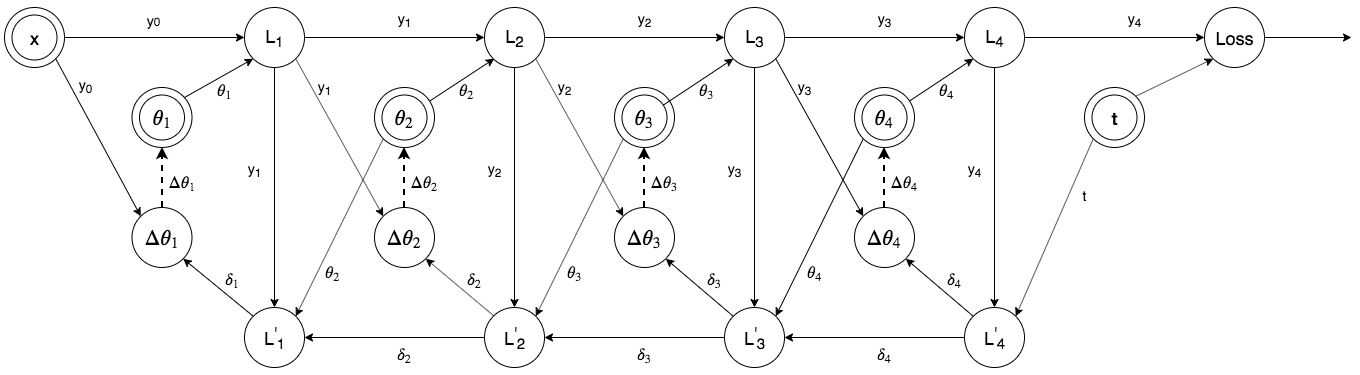
\includegraphics[width=0.97\linewidth]{backprop_full_comp_graph.png}
    \caption{The computational graph for one step of gradient descent on a neural network of four layers.}
    \label{fig:2-nn-comp-graph}
\end{figure}

\subsection{Beyond Feedforwad Networks}
In recent years, thanks to a number of breakthrough papers, certain non-linear architectures have become extremely popular, especially in vision-related tasks.
In particular, Inception modules use a split-merge architecture \cite{Szegedy2015-inception, Szegedy2016-inception-res}; and residual blocks \cite{He2016-resnet, Xie2017-resnext, Szegedy2016-inception-res} and dense blocks \cite{Huang2017-densenet} use skip connections.
These non-linearities are visualised in Figure \ref{fig:2-non-linearities}.
\begin{figure}[hbtp]
    \centering
    \hspace{0.2cm}
    \begin{subfigure}[]{0.33\textwidth}
        \centering
        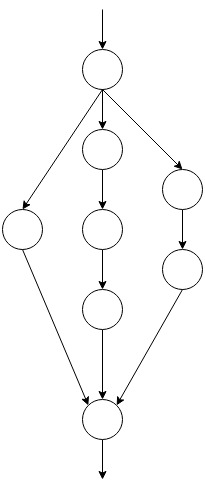
\includegraphics[height=5cm]{split-merge.jpg}
        \caption{A split-merge unit \cite{Szegedy2015-inception, Szegedy2016-inception-res}.}
    \end{subfigure}%
    \hfill
    \begin{subfigure}[]{0.30\textwidth}
        \centering
        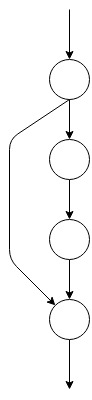
\includegraphics[height=5cm]{residual_unit.jpg}
        \caption{A residual unit \cite{He2016-resnet, Xie2017-resnext, Szegedy2016-inception-res}.}
    \end{subfigure}%
    \hfill
    \begin{subfigure}[]{0.33\textwidth}
        \centering
        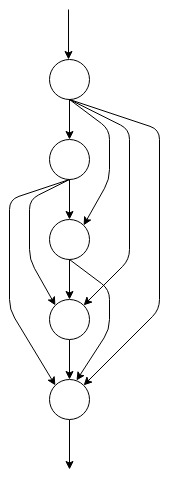
\includegraphics[height=5cm]{dense_block.jpg}
        \caption{A dense unit \cite{Huang2017-densenet}.}
    \end{subfigure}%
    \hspace{0.2cm}
    \caption{Common non-linearities in neural networks.}
    \label{fig:2-non-linearities}
\end{figure}

Recurrent Neural Networks (RNNs) also see wide use.
RNNs are networks whose output feed back into their input.
The part of the output that that feeds back to the cell is known as the \textit{hidden state}.
The cell can then be unrolled over many time steps, creating a feedforward network of RNN cells, where each cell propagates a hidden state to the next.
Such networks are trained through the Backpropagation Through Time (BPTT) algorithm \cite{Robinson1987-rnn, Mozer1989-bptt, Werbos1990-bptt}.
An example RNN cell is visualised in Figure \ref{fig:2-rnn-cell}.
\begin{figure}[h]
    \centering
    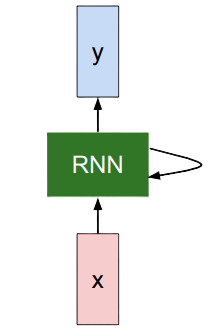
\includegraphics[width=0.22\linewidth]{rnn_cell.png}
    \caption{An RNN cell \cite[p.~22]{cs231n-rnns}.}
    \label{fig:2-rnn-cell}
\end{figure}

Unfolding this for \(t\) time steps can be visualised as in Figure \ref{fig:2-rnn-unfolded}.
Note that the same cell \(f_W\) with the same parameters \(W\) are used at each time step.

\begin{figure}[h]
    \centering
    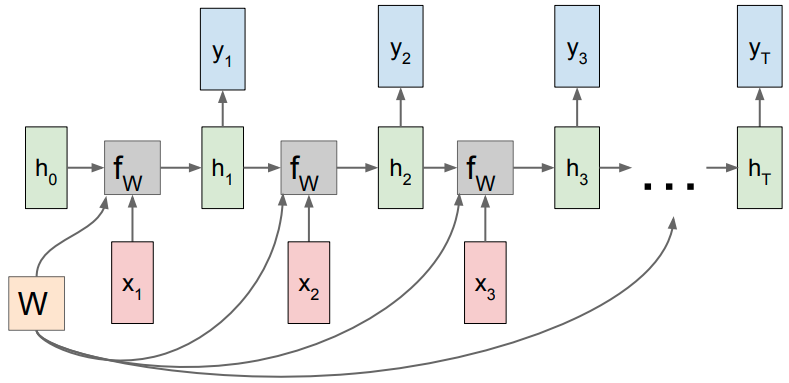
\includegraphics[width=0.7\linewidth]{rnn_unrolled.png}
    \caption{An RNN cell unrolled for \(T\) time steps \cite[p.~29]{cs231n-rnns}.}
    \label{fig:2-rnn-unfolded}
\end{figure}
In this example, we are using a \texttt{seq2seq} model.
These map a variable-sized input sequence to a variable-sized output sequence.
An example use case is natural language translation \cite{GoogleAI-mt}.
